\section{Tests}
\subsection{Förderband}
\begin{tabular}{p{3.6cm}p{\textwidth-3.6cm-0.7cm}}
    \rule{0pt}{11pt}\textit{Typ}              & Förderband\\ 
    \rule{0pt}{11pt}\textit{Datum}:           & 13.03.2015   \\
    \rule{0pt}{11pt}\textit{Ort}:             & Werkstatt \\
    \rule{0pt}{11pt}\textit{Tester}:          & Pascal Roth und Matteo Trachsel  \\
    \rule{0pt}{11pt}\textit{Ziel des Testes}: & Das Ziel des Testes besteht darin, verschieden Führungsschaufeln zu testen und eine geeignete Befetigung zu finden. \\


    \rule{0pt}{11pt}\textit{Aufbau / Ablauf}: & 
    Für den Test wurden aus einem 1 mm dicken Aluminiumblech, welches bereits auf die Breite des Förderbandes zugeschnitten wurde, verschieden Lange Stücke abgeschnitten. Da pro Tennisball zwei Führungsschaufeln vorne und hinten benötigt werden, gibt es zwei Möglichkeiten zur Gestaltung der Führungsschaufeln. Die erste Möglichkeit besteht darin, dass immer eine einzelne Schaufel für je vorne und hinten realisiert wird. Die zweite Möglichkeit besteht darin, dass man die hinter und die nächste vorne liegende Führungschaufel zusammen in einem Blechstück realisiert.\\


    \rule{0pt}{11pt}\textit{Fazit / Verbesserungs-\newline vorschlag}: & 
    Mit dem Versuch konnte gezeigt werden, dass der Kleber sicher glasklar bleibt. Weiter 
    ist die erwünschte Klebekraft bestätigt worden. Beim zweiten Versuch, wo zuerst der 
    Kleber etwas angetrocknet wurde, ist eine deutlich schlechtere Klebekraft festgestellt 
    worden. Dadurch wird der Kleber immer sofort aufgeklebt.\\
\end{tabular}

\begin{figure}[h!]
	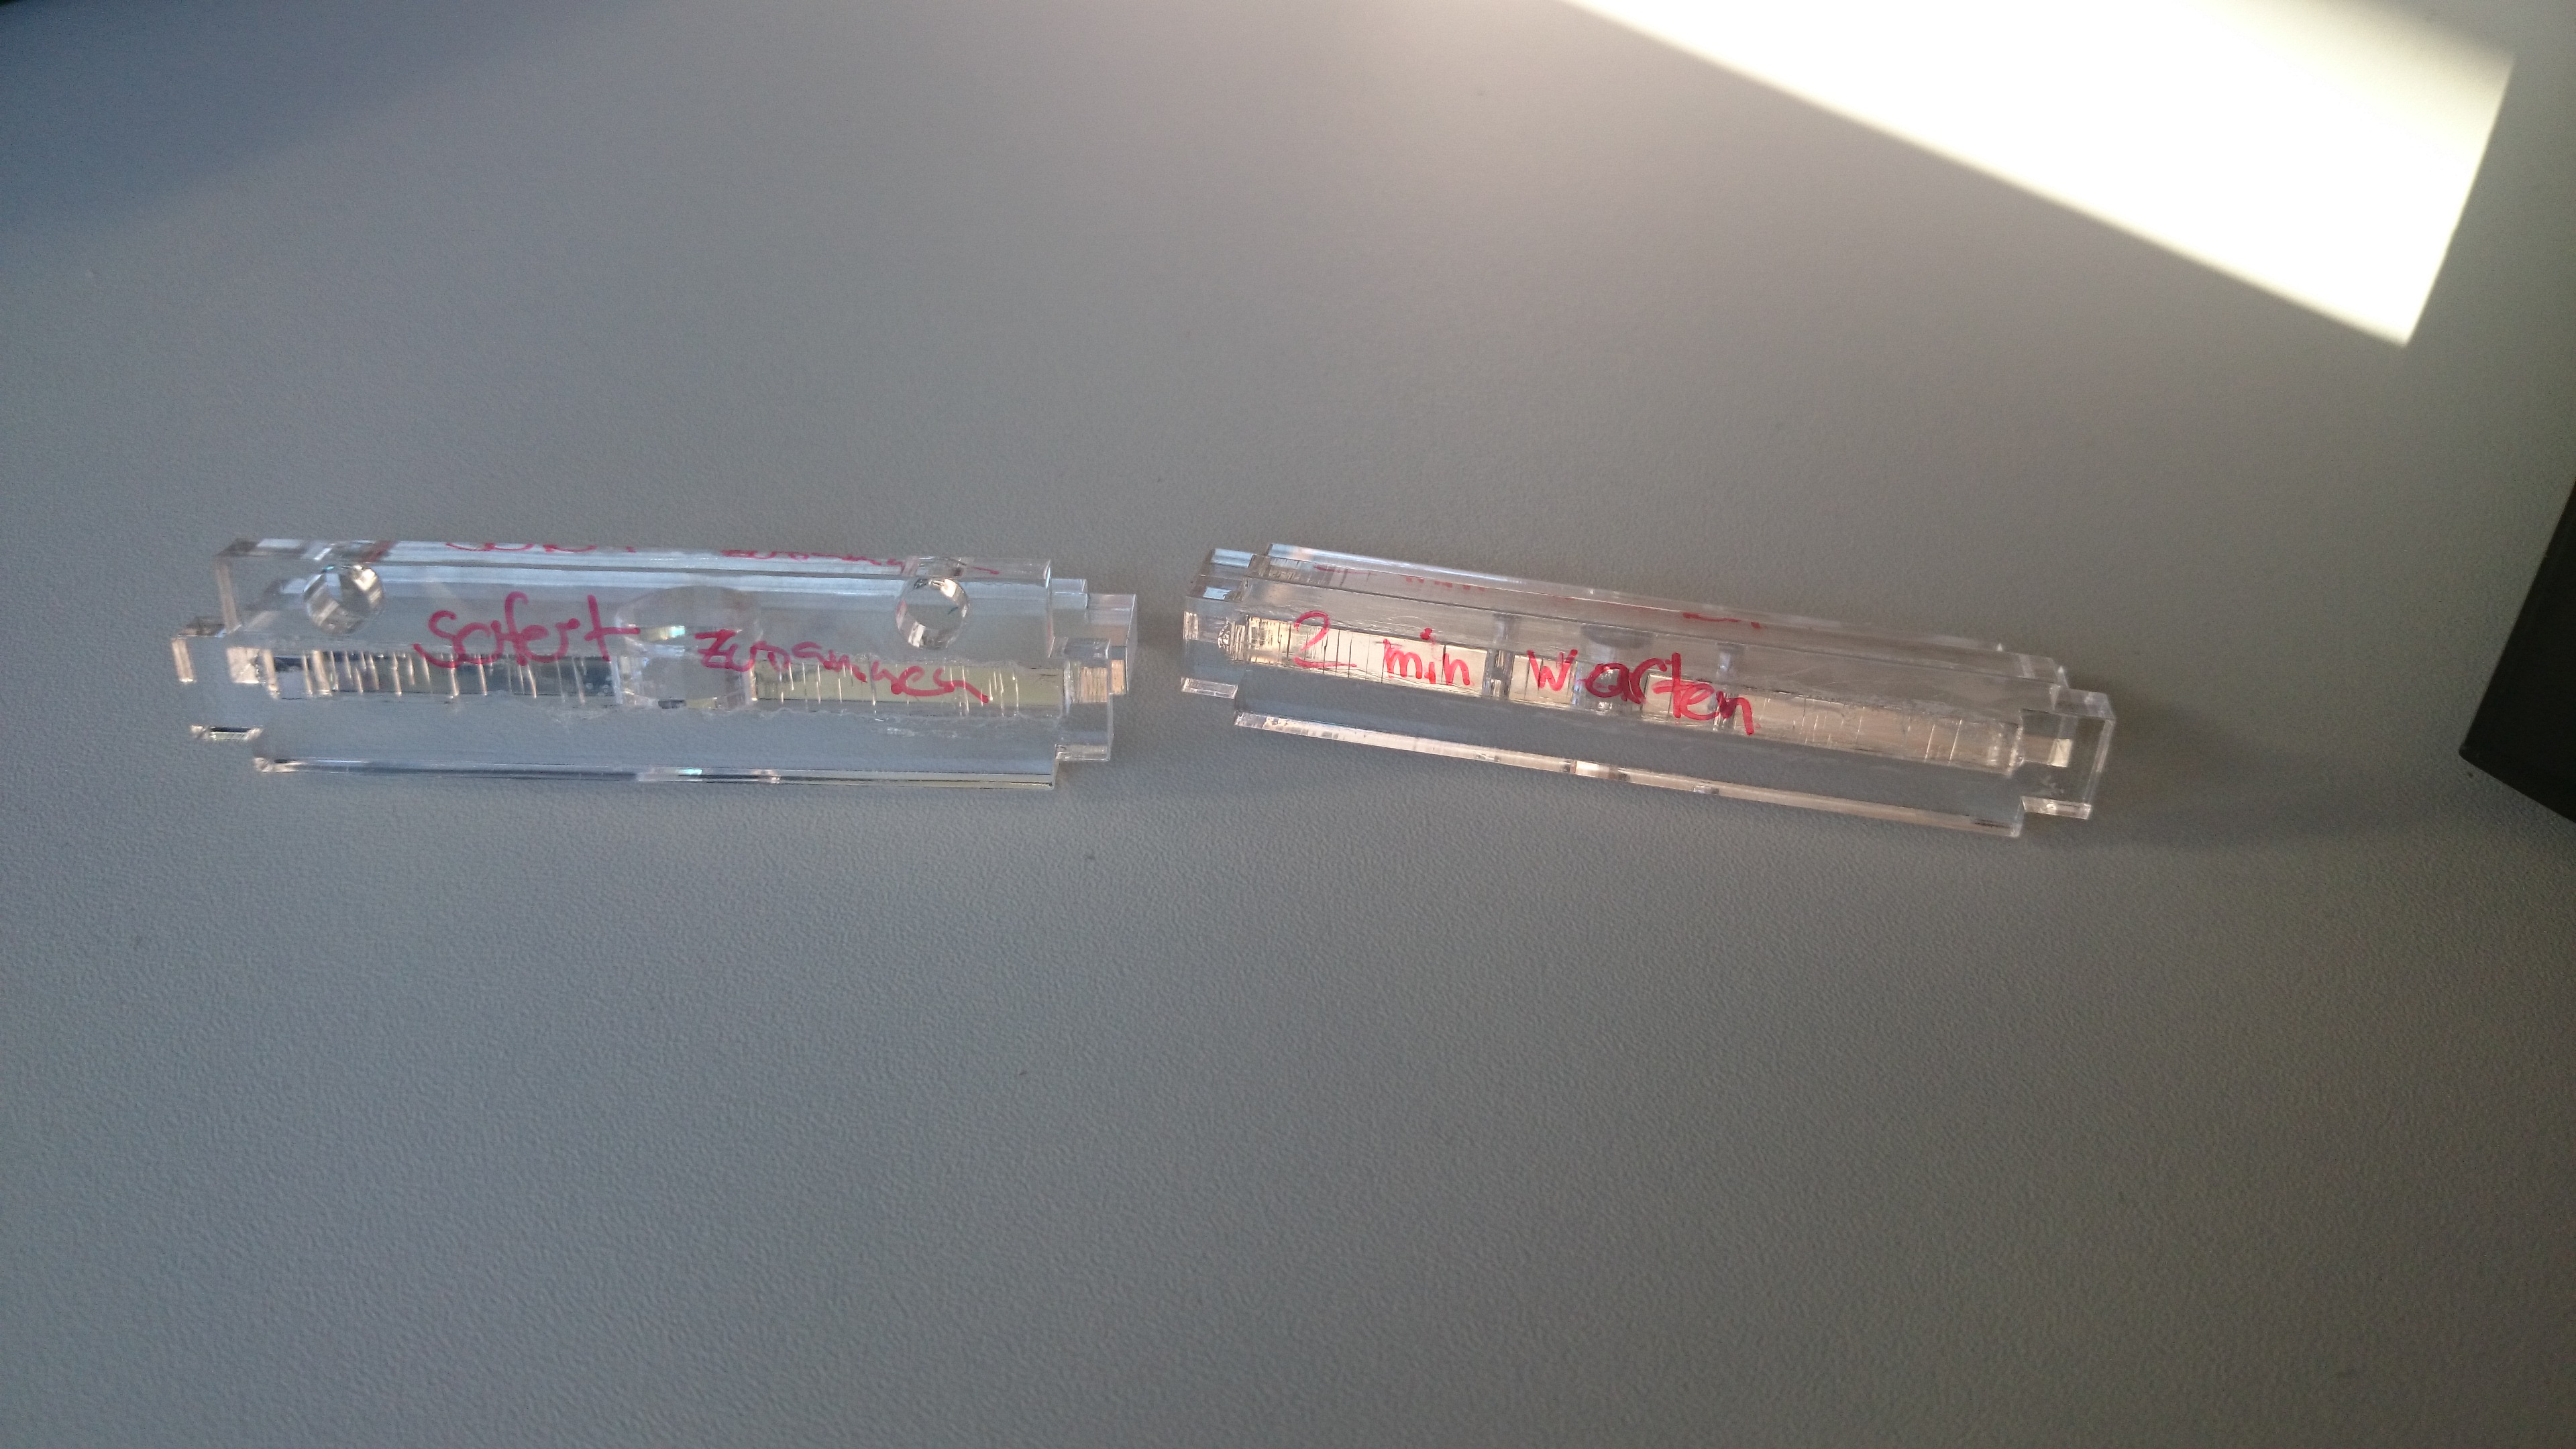
\includegraphics[width=0.9\textwidth,clip,trim=10cm 15cm 40cm 6cm]
	{Testberichte/Klebeversuch.jpg}
	\centering
	\caption{Klebeversuch mit UHU Kleber} 
	\label{abb:Klebeversuch}
\end{figure}